\ylDisplay{Tsüklotron} % Ülesande nimi
{Kristian Kuppart} % Autor
{piirkonnavoor} % Voor
{2018} % Aasta
{G 10} % Ülesande nr.
{6} % Raskustase
{
% Teema: Magnetism
\ifStatement
\begin{wrapfigure}{r}{0.35\linewidth}
	\begin{center}
		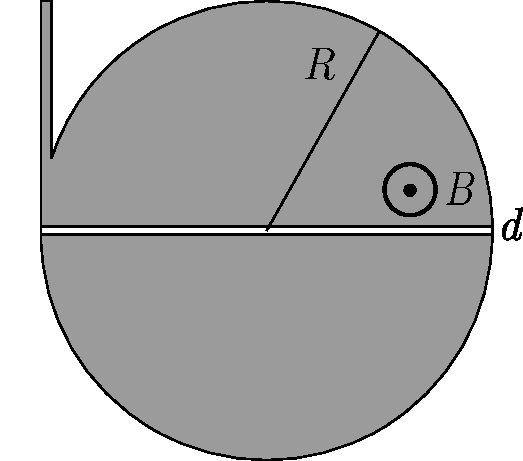
\includegraphics[width=\linewidth]{2018-v2g-10-tsyklotron}
	\end{center}
\end{wrapfigure}

Vaatleme tsüklotroni -- teatud tüüpi osakestekiirendi toimimist. Tsüklotron koosneb silindrikujulisest piirkonnast raadiusega $R$, kus on homogeenne magnetväli tugevusega $B$, ning õhukesest ribakujulisest piirkonnast laiusega $d$, kus on homogeenne ribaga risti olev elektriväli tugevusega $E$. Elektrivälja suunda muudetakse perioodiliselt vastassuunaliseks nii, et osakeste igal riba läbimisel on elektrivälja suund osakeste kiirusvektoriga samasuunaline. Samuti on tsüklotroni ühes ääres osakeste tsüklotronist väljumiseks kitsas kanal. Alustagu osakesed liikumist tsüklotroni keskelt tühiselt väikse algkiirusega. Mitu täisringi $n$ teevad osakesed tsüklotronis enne väljumist? Osakeste laeng on $q$ ja mass $m$. Eeldada, et $n\gg 1.$
\fi


\ifHint
Osakesed hakkavad tsüklotronis liikuma päripäeva mööda järjest suureneva raadiusega poolringjooni. Osake väljub tsüklotronist, kui tema trajektoori raadius kasvab sama suureks tsüklotroni raadiusega $R$.
\fi


\ifSolution
Osakesed hakkavad tsüklotronis liikuma päripäeva mööda järjest suureneva raadiusega poolringjooni. Osakese trajektoori raadius avaldub kui $r=mv/qB$, kus $v$ on osakese kiirus. Osake väljub tsüklotronist, kui tema trajektoori raadius kasvab sama suureks tsüklotroni raadiusega $R$, sel juhul tema kiirus $v=qBR/m$. Ühe täisringi jooksul saab osake elektriväljalt kineetilise energia $\varepsilon_k=2qEd$, kuna osake läbib selle aja jooksul riba 2 korda. Seega on osakese kiirus tsüklotronist väljumisel
\[\frac{mv^2}{2}=2qEdn, \qquad v^2=\frac{4qEdn}{m}.\]
Avaldades neist võrranditest $n$, saame $\displaystyle n=\frac{qB^2R^2}{4mEd}$.
\fi


\ifEngStatement
% Problem name: Cyclotron
\begin{wrapfigure}{r}{0.35\linewidth}
	\begin{center}
		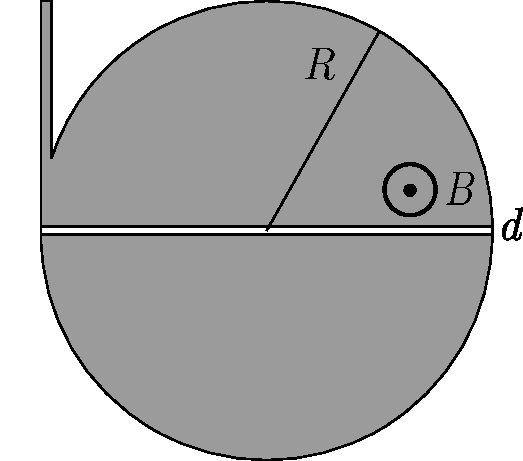
\includegraphics[width=\linewidth]{2018-v2g-10-tsyklotron}
	\end{center}
\end{wrapfigure}
Let us look at a cyclotron (a certain type of particle accelerator) and its activity. The cyclotron consists of a cylindrical region of radius $R$ where there is a homogeneous magnetic field of strength $B$ and a thin strip-shaped region of width $d$ where there is a homogenous electric field of strength $E$ perpendicular to the strip. The direction of the electrical field is changed periodically to be the opposite direction so that for every particle going through the strip the direction of the electric field is the same as the direction of the particle’s velocity. There is also a narrow canal at one edge of the cyclotron for the particles to exit the cyclotron. Let the particles start their movement at the center of the cyclotron with an insignificantly small initial speed. How many full circles $n$ will the particles make before leaving the cyclotron? The charge of the particles is $q$ and the mass $m$. Assume that $n\gg 1.$.
\fi


\ifEngHint
The particles start to move in the cyclotron clockwise along semicircles with continuously increasing radius. A particle exits the cyclotron when its trajectory radius gets as big as the radius of the cyclotron $R$.
\fi


\ifEngSolution
In the cyclotron the particles start to move clock-wise along a circle with a continuously increasing half circles. The radius of a particle is expressed as $r=mv/qB$ where $v$ is the particle’s velocity. The particle leaves the cyclotron when its trajectory radius gets as big as the cyclotron’s radius $R$, in this case its velocity is $v=qBR/m$. During one full circle the particle gets a kinetic energy from $\varepsilon_k=2qEd$ the electric field, because the particle goes through the strip two times during this time. Therefore the velocity of the particle when exiting the cyclotron is
\[\frac{mv^2}{2}=2qEdn, \qquad v^2=\frac{4qEdn}{m}.\]
Expressing $n$ from these equations we get $\displaystyle n=\frac{qB^2R^2}{4mEd}$.
\fi
}